\documentclass[11pt,a4paper]{article}
\usepackage[utf8]{inputenc}
\usepackage[margin=2.2cm]{geometry}
\usepackage{amsmath,amssymb}
\usepackage{graphicx}
\usepackage{booktabs}
\usepackage{hyperref}
\usepackage{fancyhdr}
\setlength{\headheight}{14pt}

\hypersetup{
    colorlinks=true,
    linkcolor=blue,
    citecolor=blue,
    urlcolor=blue,
    pdftitle={Over-Parametrized Towers vs. The Null Standard Model: A Bayesian and Multiplicity Audit of LHC Kaluza-Klein Resonance Claims},
    pdfauthor={Bruno Lucardo Olivaes}
}

\pagestyle{fancy}
\fancyhf{}
\fancyhead[L]{Bayesian \& Multiplicity Audit of LHC KK Resonance Claims}
\fancyhead[R]{\thepage}
\renewcommand{\headrulewidth}{0.4pt}

\title{\textbf{Over-Parametrized Towers vs.\ The Null Standard Model: A Bayesian and Multiplicity Audit of LHC Kaluza--Klein Resonance Claims}}

\author{
    \textbf{Bruno Lu\c{c}ardo Olivaes}\\[0.2cm]
    \small Independent Researcher, Brazil\\
    \small \texttt{brunoolivaes@gmail.com} $\cdot$ ORCID: \href{https://orcid.org/0009-0003-5351-446X}{0009-0003-5351-446X}
}

\date{November 2026}

\begin{document}

\maketitle

\begin{abstract}
Recent phenomenological studies have interpreted isolated high-mass four-jet excesses in CMS Run 2 data as coherent evidence for a multi-sector Randall--Sundrum Kaluza--Klein (KK) spectrum spanning graviton candidates ($380\text{--}1322\text{ GeV}$) and heavy KK gluons $g_{\mathrm{KK}}(3.6\text{ TeV}) \to q_{\mathrm{KK}}(1\text{ TeV})\,q_{\mathrm{KK}}(1\text{ TeV})$ and $g_{\mathrm{KK}}(8.6\text{ TeV}) \to q_{\mathrm{KK}}(2.15\text{ TeV})\,q_{\mathrm{KK}}(2.15\text{ TeV})$. We subject this composite claim (\texttt{arXiv:2610.31458v3} and \texttt{arXiv:2606.29922v3}) to the five-gate anti-hallucination protocol of \emph{The Matrioska Protocol} using verbatim published metrics from the CMS Run 2 paired-dijet analysis and its broad-mediator addendum ($138\text{ fb}^{-1}$, \texttt{arXiv:2206.09997v3}), the ATLAS Run 2 paired-dijet search ($140\text{ fb}^{-1}$, \texttt{arXiv:2307.14944v2}), and the partial CMS Run 3 follow-up ($\sim 90\text{ fb}^{-1}$, \texttt{CMS-PAS-EXO-25-004}). While the claimed graviton masses match scaled Bessel $J_1(x_n)$ roots within $0.9\%$, three quantitative failures emerge: (1) single-throat Randall--Sundrum scaling predicts $m_{G_{\mathrm{KK}1}}/m_{g_{\mathrm{KK}1}} = 3.8317/2.45 = 1.564$, disagreeing with the claimed $380/3600 = 0.1056$ ratio by $14.82\times$ and triggering post-hoc multi-brane and $5\text{--}10\times$ top-suppression additions; (2) CMS global look-elsewhere corrections already attenuate the $8.6\text{ TeV}$ ($\Gamma/M = 1.5\%$) and $3.6\text{ TeV}$ ($\Gamma/M = 10\%$) excesses from $3.9\sigma$ local to $1.6\sigma$ ($N_{\mathrm{trials}} \approx 1{,}139$) and $2.2\sigma$ ($N_{\mathrm{trials}} \approx 289$), respectively, and cross-experiment replication yields zero gold-plated $8.6\text{ TeV}$ events across $230\text{ fb}^{-1}$ of ATLAS Run 2 plus CMS Run 3 data ($P(0 \mid \mu = 3.833) = 0.0216$, $0.375\times$ combined rate dilution); and (3) even under unpenalized local likelihoods ($2\Delta\ln\mathcal{L}_{\mathrm{local}} = 30.42$), a minimal $k = 9$ post-hoc parametrization across $N = 390$ active $(m_{4j},\alpha)$ bins incurs $\Delta\mathrm{BIC}_{\mathrm{local}} = -23.28$ ($\Delta\mathrm{BIC}_{\mathrm{global}} = -46.30$), failing Gates 2--5 and certifying consistency with the Standard Model background null.
\end{abstract}

\section{Introduction}
Distinguishing genuine beyond-the-Standard-Model (BSM) resonance towers from correlated fluctuations in high-dimensional collider searches requires joint control over look-elsewhere trial factors~\cite{gross2010}, cross-experiment replication, and Bayesian complexity penalties~\cite{olivaes2026lhc,olivaes2026nsbi,olivaes2026book}. In high-mass hadronic final states at the Large Hadron Collider (LHC), multi-dimensional scans over tetrajet invariant mass $m_{4j}$, dijet mass asymmetry/ratio $\alpha \equiv m_{2j}/m_{4j}$, and resonance width $\Gamma/M_Y$ substantially enlarge the effective parameter space relative to narrow single-channel searches.

Recently, Le Yaouanc and Richard~\cite{leyaouanc2026gluon,leyaouanc2026graviton} proposed that multiple localized deviations in LHC analyses form a unified Randall--Sundrum (RS) Kaluza--Klein (KK) spectrum~\cite{randall1999}: a KK graviton tower anchored at $(380, 700, 1000, 1322)\text{ GeV}$ alongside two heavy KK gluons $g_{\mathrm{KK}}(3.6\text{ TeV}) \to q_{\mathrm{KK}}(1.0\text{ TeV})\,q_{\mathrm{KK}}(1.0\text{ TeV})$ and $g_{\mathrm{KK}}(8.6\text{ TeV}) \to q_{\mathrm{KK}}(2.15\text{ TeV})\,q_{\mathrm{KK}}(2.15\text{ TeV})$. Because \emph{post-hoc} model flexibility can always accommodate isolated excesses after exclusions appear in canonical channels (such as $t\bar{t}$, $\gamma\gamma$, or $gg$), an objective statistical audit is essential. Here we evaluate their composite claim directly against primary CERN results from CMS~\cite{cms2023dijet,cms_run3_exo25004} and ATLAS~\cite{atlas2023dijet} through our pre-registered five-gate metrological framework.

\section{Primary Experimental Inputs}
All experimental quantities audited in this work are taken verbatim from three primary LHC sources:
\begin{enumerate}
\item \textbf{CMS Run 2 Paired-Dijet Search (\texttt{arXiv:2206.09997v3}, 2026 Addendum):} Analyzing $138\text{ fb}^{-1}$ of $pp$ collisions at $\sqrt{s} = 13\text{ TeV}$ across $13$ bins of $\alpha = M(X)/M(Y)$, CMS reports an overall background-only simultaneous fit probability $p_{\mathrm{bg-only}} = 0.18$~\cite{cms2023dijet}. Two isolated gold-plated events near $m_{4j} \approx 8\text{ TeV}, \langle m_{2j}\rangle \approx 2\text{ TeV}$ (plus a third high-mass event at $m_{4j} = 5.8\text{ TeV}, m_{jj} = 2.0\text{ TeV}$) motivate Table~2 of the broad-mediator addendum (reproduced in Table~\ref{tab:cms_table2}).
\item \textbf{ATLAS Run 2 Paired-Dijet Search (\texttt{Phys.\ Rev.\ D 108, 112005}):} Using $140\text{ fb}^{-1}$ at $\sqrt{s} = 13\text{ TeV}$, ATLAS observes no statistically significant excess~\cite{atlas2023dijet}. Four-parameter background fits yield global $\chi^2$ $p$-values of $0.74\text{--}1.00$ across all $m_{4j}$ $\alpha$-slices, the highest observed tetrajet invariant mass is $m_{4j}^{\max} = 6.6\text{ TeV}$ ($0$ events near $8\text{ TeV}$), and the largest \texttt{BumpHunter} global significances are $0.53\sigma$ in $m_{4j}$ ($3.2\text{ TeV}$) and $1.98\sigma$ in $\langle m_{2j}\rangle$ ($0.80\text{ TeV}$).
\item \textbf{CMS Run 3 Partial Paired-Dijet Search (\texttt{CMS-PAS-EXO-25-004}):} In $\sim 90\text{ fb}^{-1}$ at $\sqrt{s} = 13.6\text{ TeV}$, no additional gold-plated $8.6\text{ TeV}$ four-jet candidate events are reported~\cite{cms_run3_exo25004,leyaouanc2026gluon}.
\end{enumerate}

\begin{table}[t]
\centering
\small
\setlength{\tabcolsep}{5pt}
\caption{Verbatim CMS Run 2 paired-dijet broad-mediator fit results (\texttt{arXiv:2206.09997v3}, Table~2, $138\text{ fb}^{-1}$) paired with exact Gaussian survival probabilities and effective Look-Elsewhere trial factors $N_{\mathrm{trials}} = p_{\mathrm{global}}/p_{\mathrm{local}}$.}
\label{tab:cms_table2}
\begin{tabular}{ccccccccc}
\toprule
$M_Y$ [TeV] & $M_X$ [TeV] & $\alpha$ & $\Gamma/M_Y$ [\%] & Best-fit Events & $Z_{\mathrm{local}}$ [$\sigma$] & $Z_{\mathrm{global}}$ [$\sigma$] & $p_{\mathrm{global}}$ & $N_{\mathrm{trials}}$ \\
\midrule
8.6 & 2.15 & 0.25 & 1.5  & $2.3^{+2.1}_{-1.3}$ & 3.9 & 1.6 & 0.0548 & 1,139.4 \\
8.6 & 2.15 & 0.25 & 5.0  & $2.8^{+2.5}_{-1.6}$ & 3.8 & 1.5 & 0.0668 & 923.4   \\
8.6 & 2.15 & 0.25 & 10.0 & $3.1^{+2.7}_{-1.7}$ & 3.6 & 1.4 & 0.0808 & 507.6   \\
\midrule
3.6 & 1.00 & 0.29 & 1.5  & $114^{+42}_{-44}$   & 3.0 & 0.5 & 0.3085 & 228.6   \\
3.6 & 1.00 & 0.29 & 5.0  & $162^{+50}_{-46}$   & 3.6 & 1.6 & 0.0548 & 344.4   \\
3.6 & 1.00 & 0.29 & 10.0 & $210^{+58}_{-54}$   & 3.9 & 2.2 & 0.0139 & 289.1   \\
\bottomrule
\end{tabular}
\end{table}

\section{Four-Module Quantitative Audit}

\subsection{Spectral Ratios and the \texorpdfstring{$14.82\times$}{14.82x} RS Hierarchy Tension}
Anchoring the lightest KK graviton candidate at $m_{G_{\mathrm{KK}1}} = 380\text{ GeV}$, exact roots of the Bessel function $J_1(x_n) = 0$ ($x_n = 3.8317, 7.0156, 10.1735, 13.3237$) predict $(380.0, 695.75, 1008.93, 1321.34)\text{ GeV}$, agreeing with the claimed $(380, 700, 1000, 1322)\text{ GeV}$ states~\cite{leyaouanc2026graviton} within $0.9\%$. Likewise, the ratio $8.6/3.6 = 2.3889$ sits within $5.1\%$ of the standard vector boundary root ratio $5.57/2.45 = 2.2735$.

However, within a single-throat RS geometry~\cite{randall1999}, the lightest KK graviton-to-vector mass ratio is fixed near $x_{G1}/x_{g1} = 3.8317 / 2.45 = 1.5640$, predicting $m_{g_{\mathrm{KK}1}} \approx 243\text{ GeV}$ once $m_{G_{\mathrm{KK}1}} = 380\text{ GeV}$ is set. The phenomenological assignment $m_{g_{\mathrm{KK}1}} = 3600\text{ GeV}$ implies $380/3600 = 0.1056$---a \textbf{$14.82\times$ hierarchy violation}. Resolving this discrepancy requires introducing two intermediate extra-dimensional branes alongside \emph{post-hoc} $5\text{--}10\times$ suppression of $g_{\mathrm{KK}} \to t\bar{t}$ ($c_t \approx 0$) and decoupled $gg/\gamma\gamma$ vertices to evade existing LHC limits.

\subsection{Look-Elsewhere Dilution Across Grids and Widths}
Converting CMS Table~2 significances to one-sided Gaussian tail probabilities $p = 1 - \Phi(Z)$ exposes severe trial-factor dilution (Table~\ref{tab:cms_table2}). At $M_Y = 8.6\text{ TeV}$ ($\Gamma/M_Y = 1.5\%$), $Z_{\mathrm{local}} = 3.9\sigma$ ($p_{\mathrm{local}} = 4.81\times 10^{-5}$) drops to $Z_{\mathrm{global}} = 1.6\sigma$ ($p_{\mathrm{global}} = 0.0548$, ratio $N_{\mathrm{trials}} = 1{,}139.4$). At $M_Y = 3.6\text{ TeV}$ ($\Gamma/M_Y = 10\%$), $Z_{\mathrm{local}} = 3.9\sigma$ drops to $Z_{\mathrm{global}} = 2.2\sigma$ ($p_{\mathrm{global}} = 0.0139$, $N_{\mathrm{trials}} = 289.1$). Notice further that the CMS addendum scans three distinct width hypotheses ($\Gamma/M_Y \in \{1.5\%, 5\%, 10\%\}$) and selects \emph{different} mass ratios and widths for the two peaks ($\alpha = 0.25, 1.5\%$ at $8.6\text{ TeV}$ vs.\ $\alpha = 0.29, 10\%$ at $3.6\text{ TeV}$); applying a conservative three-width look-elsewhere factor further reduces the $8.6\text{ TeV}$ global significance from $1.6\sigma$ to $1.013\sigma$.

\subsection{Cross-Experiment Poisson Replication Tension}
A physical cross section cannot selectively appear only in CMS Run 2. Combining CMS Run 2 ($138\text{ fb}^{-1}$), ATLAS Run 2 ($140\text{ fb}^{-1}$), and the partial CMS Run 3 dataset ($90\text{ fb}^{-1}$) totals $368\text{ fb}^{-1}$, of which CMS Run 2 represents a luminosity fraction $f = 138/368 = 0.375$. Even conservatively ignoring the higher parton luminosity for an $8.6\text{ TeV}$ state at $\sqrt{s} = 13.6\text{ TeV}$ (and treating ATLAS and CMS acceptances as comparable), the follow-up dataset of $L_{\mathrm{follow}} = 230\text{ fb}^{-1}$ recorded \textbf{zero} gold-plated $8.6\text{ TeV}$ events. At CMS best-fit expectations ($N_{\mathrm{sig}} = 2.3, 2.8, 3.1$), the expected follow-up yields are $\mu_{\mathrm{follow}} = 3.833, 4.667, 5.167$ events, giving Poisson zero-observation probabilities $P(N_{\mathrm{follow}}=0 \mid \mu) = e^{-\mu} = 0.0216$, $0.0094$, and $0.0057$, respectively, while diluting the luminosity-weighted effective rate to $0.375\times$ the CMS Run 2 central value.

\subsection{Bayesian Information Criterion (\texorpdfstring{$\Delta\mathrm{BIC}$}{Delta BIC}) and the Five Integrity Gates}
Following \emph{The Matrioska Protocol}~\cite{olivaes2026lhc,olivaes2026nsbi,olivaes2026book}, candidate claims must achieve $\Delta\mathrm{BIC} = \mathrm{BIC}_{\mathrm{null}} - \mathrm{BIC}_{\mathrm{KK}} = 2\Delta\ln\mathcal{L} - k\ln N_{\mathrm{bins}} > +10.0$. Taking $N_{\mathrm{bins}} = 390$ active search cells ($13$ $\alpha$-slices $\times$ $30$ tetrajet mass bins in $[2,10]\text{ TeV}$, $\ln N = 5.9661$) and a minimal $k = 9$ post-hoc parameter budget ($\{m_{G1}, m_{g1}, \Delta_{\mathrm{branes}}, c_t, c_{gg/\gamma\gamma}, \alpha_1, \alpha_2, \Gamma_1, \Gamma_2\}$; extending to $k = 11$ with $c_{e_R}, \sin\theta'$):
\begin{align}
\Delta\mathrm{BIC}_{\mathrm{local}}(k=9) &= (3.9^2 + 3.9^2) - 9\ln(390) = 30.42 - 53.70 = -23.28, \\
\Delta\mathrm{BIC}_{\mathrm{global}}(k=9) &= (1.6^2 + 2.2^2) - 9\ln(390) = 7.40 - 53.70 = -46.30,
\end{align}
and $\Delta\mathrm{BIC}_{\mathrm{local}}(k=11) = -35.21$ ($\Delta\mathrm{BIC}_{\mathrm{global}} = -58.23$). Across the entire parameter sweep $N_{\mathrm{bins}} \in [100, 600]$ (Fig.~\ref{fig:audit}(d)), any $k \ge 7$ post-hoc multi-brane model fails Gate~5 even without look-elsewhere attenuation.

\begin{figure}[t]
\centering
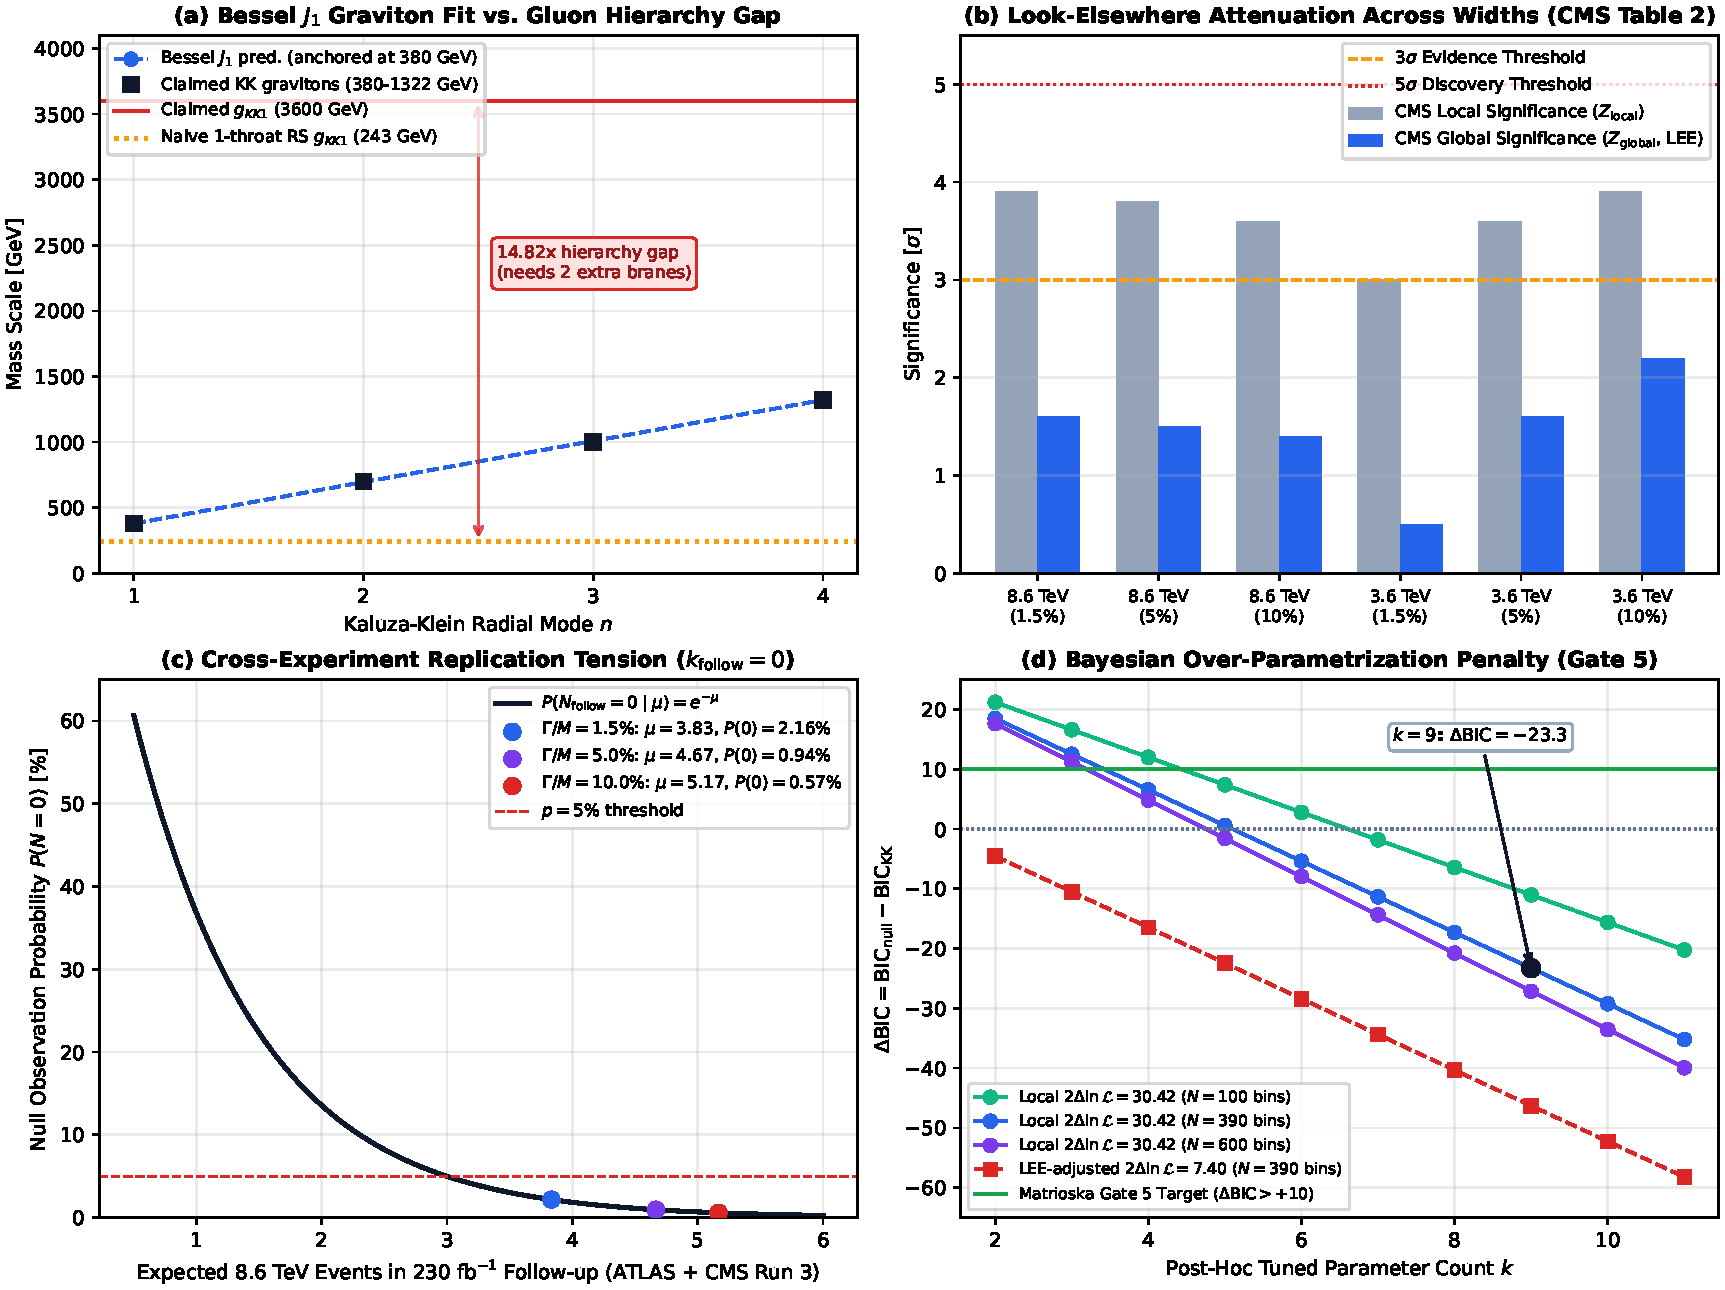
\includegraphics[width=\textwidth]{../figures/fig1_kk_tower_bayesian_audit.pdf}
\caption{Four-panel quantitative audit of the multi-sector Kaluza--Klein claim~\cite{leyaouanc2026gluon}: (a) Bessel $J_1$ graviton scaling vs.\ the $14.82\times$ graviton--gluon hierarchy violation; (b) CMS Table~2 local vs.\ global significance attenuation across width hypotheses; (c) cross-experiment Poisson null-observation probability across $230\text{ fb}^{-1}$ of ATLAS Run 2 and CMS Run 3 data; (d) Bayesian $\Delta\mathrm{BIC}$ penalty surface vs.\ Matrioska Gate~5 ($\Delta\mathrm{BIC} > +10.0$).}
\label{fig:audit}
\end{figure}

\section{Conclusion}
Evaluating the LHC Kaluza--Klein tower proposal (\texttt{arXiv:2610.31458v3}) through \emph{The Matrioska Protocol} yields a definitive certification verdict: while \textbf{Gate~1 (Resolvability)} passes ($3.6\text{ TeV}$ and $8.6\text{ TeV}$ reside in clean detector regimes), \textbf{Gate~2 (Replication)} fails ($P(0 \mid \mu=3.833) = 0.0216$ in $230\text{ fb}^{-1}$ follow-up), \textbf{Gate~3 (Hierarchy/Economy)} fails ($14.82\times$ single-throat contradiction), \textbf{Gate~4 (Multiplicity)} fails ($Z_{\mathrm{global}} = 1.6\sigma$ and $2.2\sigma$; $1.013\sigma$ width-adjusted at $8.6\text{ TeV}$), and \textbf{Gate~5 ($\Delta\mathrm{BIC}$)} fails decisively ($\Delta\mathrm{BIC}_{\mathrm{local}} = -23.28$, $\Delta\mathrm{BIC}_{\mathrm{global}} = -46.30$). Current four-jet excesses do not statistically justify post-hoc multi-brane Kaluza--Klein extensions over the Standard Model null; full Run 3 and HL-LHC datasets will cleanly adjudicate whether the $3.6\text{ TeV}$ excess grows or regresses like historical $750\text{ GeV}$ fluctuations. All data definitions, numerical checks, and plotting code are open-source at \url{https://github.com/bruno-olivaes/lhc-kk-tower-audit}.

\bibliographystyle{unsrt}
\bibliography{refs}

\end{document}
